% ========== Appendix C
 
\chapter{Frontier Comparison Metrics}
\label{chap:appCComparisonMetrics}
This chapter describes in more detail metrics used to compare Pareto frontiers.

\section{Dominance relations}
\label{sec:dominanceRelationships}
Table \ref{tab:dominanceRelations} defines the terms regarding dominance relations used here.

\begin{table}[ht]
\centering
\resizebox{\textwidth}{!}{%
\begin{tabular}{|p{.2\linewidth}|p{.1\linewidth}|p{.3\linewidth}|p{.1\linewidth}|p{.3\linewidth}|}
\hline
\textbf{Relation}           & \multicolumn{2}{c|}{\textbf{Solutions}}                                                                                                                                                                          & \multicolumn{2}{c|}{\textbf{Frontiers}}                                                                                                     \\ \hline
Strictly dominates & $\mathbf{z}^1 \succ \succ \mathbf{z}^2$ & $\forall i \in \mathcal{M}$,                                                                                 $z^1_i > z^2_i$ & $Z^1 \succ \succ Z^2$ & Every solution in $Z^2$ is strictly dominated by at least one solution in $Z^1$                  \\ \hline
Dominates          & $\mathbf{z}^1 \succ \mathbf{z}^2$       & $\forall i \in \mathcal{M}$, $z^1_i \ge z^2_i \wedge \exists i \in \mathcal{M}:  z^1_i > z^2_i$ & $Z^1 \succ Z^2$       & Every solution in $Z_2$ is dominated by at least one solution in $Z_1$                           \\ \hline
Better             &                                         &                                                                                                                                                               & $Z^1 \rhd Z^2$        & Every solution in $Z^2$ is weakly dominated by at least one solution in $Z^1$ and $Z^1 \neq Z^2$ \\ \hline
Weakly dominates   & $\mathbf{z}^1 \succeq \mathbf{z}^2$     & $\forall i \in \mathcal{M}$, $z^1_i \ge z^2_i$                                                                                        & $Z^1 \succeq Z^2$     & Every solution in $Z^2$ is weakly dominated by at least one solution in $Z^1$          \\ \hline
Incomparable       & $\mathbf{z}^1 || \mathbf{z}^2$          & Neither $\mathbf{z}^1$ nor $\mathbf{z}^2$ weakly dominates the other                                                                                          & $Z_1 || Z_2$          & Neither $Z^1$ nor $Z^2$ weakly dominates the other                                                         \\ \hline
\end{tabular}%
}
\caption[Dominance relationships for frontiers and solutions]{Definitions of dominance relationships between solutions and between frontiers, reproduced from Zitzler \textit{et al.} \cite{zitzler2003performance}.}
\label{tab:dominanceRelations}
\end{table}

\section{Additive binary epsilon indicator $I_{\epsilon_+2}$}
\label{sec:binaryEpsIndicator}
Given two frontiers, $Z^1$ and $Z^2$, the additive binary epsilon indicator is defined as in \cite{zitzler2003performance}:
\begin{align}
I_{\epsilon_+2} (Z^1,Z^2) = \inf_{\epsilon \in \mathbb{R}} \set{\forall \mathbf{z}^2 \in Z^2 \; \exists \mathbf{z}^1 \in Z^1 : \mathbf{z}^1 \succeq_{\epsilon_+} \mathbf{z}^2}
\end{align}
where $\succeq_{\epsilon_+}$ is the additive $\epsilon$-dominance relationship:
\begin{align}
\mathbf{z}^1 \succeq_{\epsilon_+} \mathbf{z}^2 \iff \epsilon + z^1_i \ge z^2_i \quad \forall 1 \le i \le M
\end{align}
Intuitively, $\epsilon$ is the minimum amount by which a frontier $Z^1$ must be translated such that every solution $\mathbf{z}^2 \in Z^2$ is ``covered''. See Figure \ref{fig:binaryEpsilon}. Positive values of $I_{\epsilon_+2} (Z^1,Z^2)$ indicate the presence of points $\mathbf{z}^2 \in Z^2$ that are not dominated by $Z^1$. Negative values of $I_{\epsilon_+2} (Z^1,Z^2)$ indicate that $Z^1$ strictly dominates $Z^2$ ($Z^1 \succ \succ Z^2$).

\begin{figure}[ht]
\centering
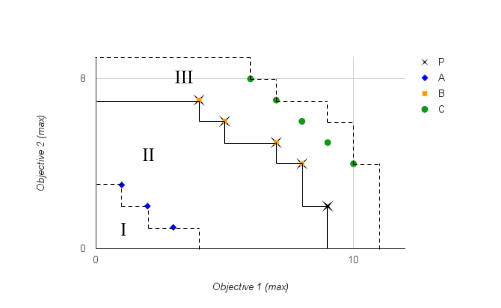
\includegraphics[width=.7\textwidth]{../images/BinaryEpsilonIndicator}
\caption[The additive binary epsilon indicator $I_{\epsilon_+2}$]{Depiction of the additive binary epsilon indicator $I_{\epsilon_+2}$ and the additive epsilon dominance relationship $\succeq_{\epsilon_+}$. In the figure,

\begin{minipage}{\linewidth}
  \begin{align*}
    I_{\epsilon_+2} (P,A) = -4 < 0 \qquad I_{\epsilon_+2} (P,B) = 0 \qquad I_{\epsilon_+2} (P,C) = 2 > 0
  \end{align*}
\end{minipage}

Region III is $\epsilon_+$-dominated for $\epsilon = 2$; region II is $\epsilon_+$-dominated for $\epsilon = 0$; region I is $\epsilon_+$-dominated for $\epsilon = -4$. Note that region II also encompasses region I, and region III encompasses region II.}
\label{fig:binaryEpsilon}
\end{figure}

\section{Additive unary epsilon indicator $I_{\epsilon_+}$}
\label{sec:unaryEpsIndicator}
I define the unary epsilon indicator as
\begin{align}
I_{\epsilon_+} (Z) = I_{\epsilon_+2} (Z,\mathbf{z}^{\text{ideal}}) \label{eqn:unaryEpsIndicator}
\end{align}
That is, the additive unary epsilon indicator is identical to the additive binary epsilon indicator where the second frontier consists of a single point: the ideal solution for the first frontier.

This differs from the unary epsilon indicator traditionally used in EMO \cite{zitzler2003performance} in which the frontier is compared against a reference nondominated set. However, because the frontiers in the present study have guaranteed optimality, there is no reference set against which to compare them.

\section{Hypervolume Indicators}
\label{sec:hypervolumeIndicator}
For every solution $\mathbf{z}^i$ in a frontier $Z$ define the hyperrectangle $r_i$ whose diagonal corners are the origin and the objective vector $\mathbf{z}^i = [z_1,\ldots,z_M]$ (see Figure \ref{fig:frontierVolumes}). Then the \textit{unary hypervolume indicator} of the frontier $Z$ is the $M$-dimensional volume of the union of all of the hyperrectangles corresponding to the solutions in $Z$:
\begin{align}
I_{H1} (Z) = \text{vol} \left( \bigcup_{i = 1}^{|Z|} r_i \right) \label{eqn:hypervol}
\end{align}
Then define the \textit{binary hypervolume indicator} of two frontiers $Z^1$ and $Z^2$ as \cite{zitzler1999evolutionary}
\begin{align}
I_{H2} (Z^1,Z^2) = I_{H1} (Z^1 + Z^2) - I_{H1} (Z^2)
\end{align}
where $I_{H1} (Z^1 + Z^2)$ is the unary hypervolume indicator of the frontier consisting of the nondominated points in $Z = \{\mathbf{z} \in Z^1 \cup Z^2\}$ . See Figure \ref{fig:binaryHypervolume}. The binary hypervolume indicator provides the volume of frontier $Z^1$ that is not contained within frontier $Z^2$. Larger values of $I_{H1}$ correspond to frontiers occupying larger amounts of the objective space. $I_{H2}(Z^1, Z^2) > I_{H2}(Z^2, Z^1)$ indicates areas of less conflict between objectives in $Z^1$ than in $Z^2$.

\begin{figure}[ht]
\centering
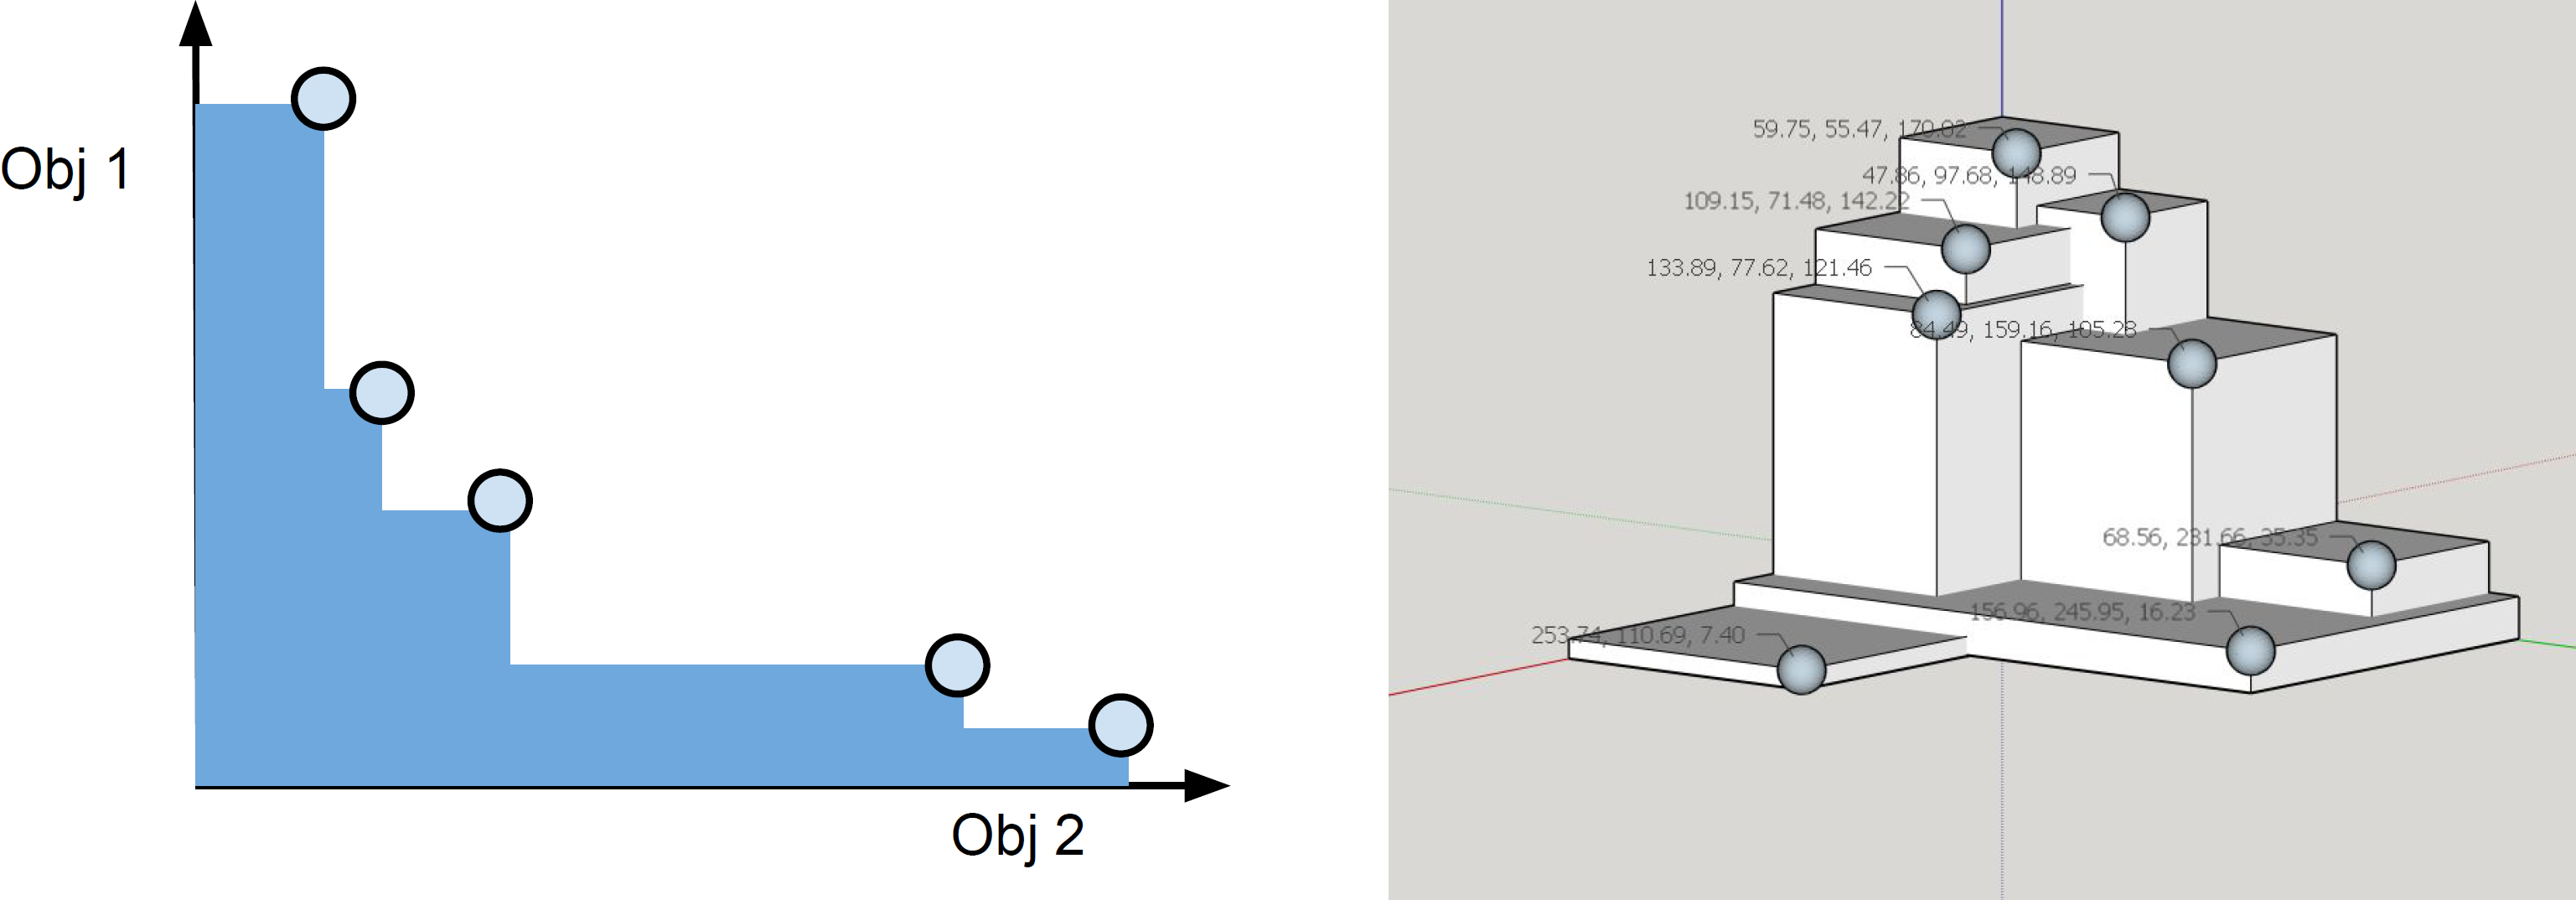
\includegraphics[width=.85\textwidth]{../images/FrontierVolumesNo2DOutlines}
\caption[Hypervolume of Pareto frontiers]{Depiction of the hypervolumes of frontiers with two objectives (left) and three objectives (right).}
\label{fig:frontierVolumes}
\end{figure}

\begin{figure}[ht!]
\centering
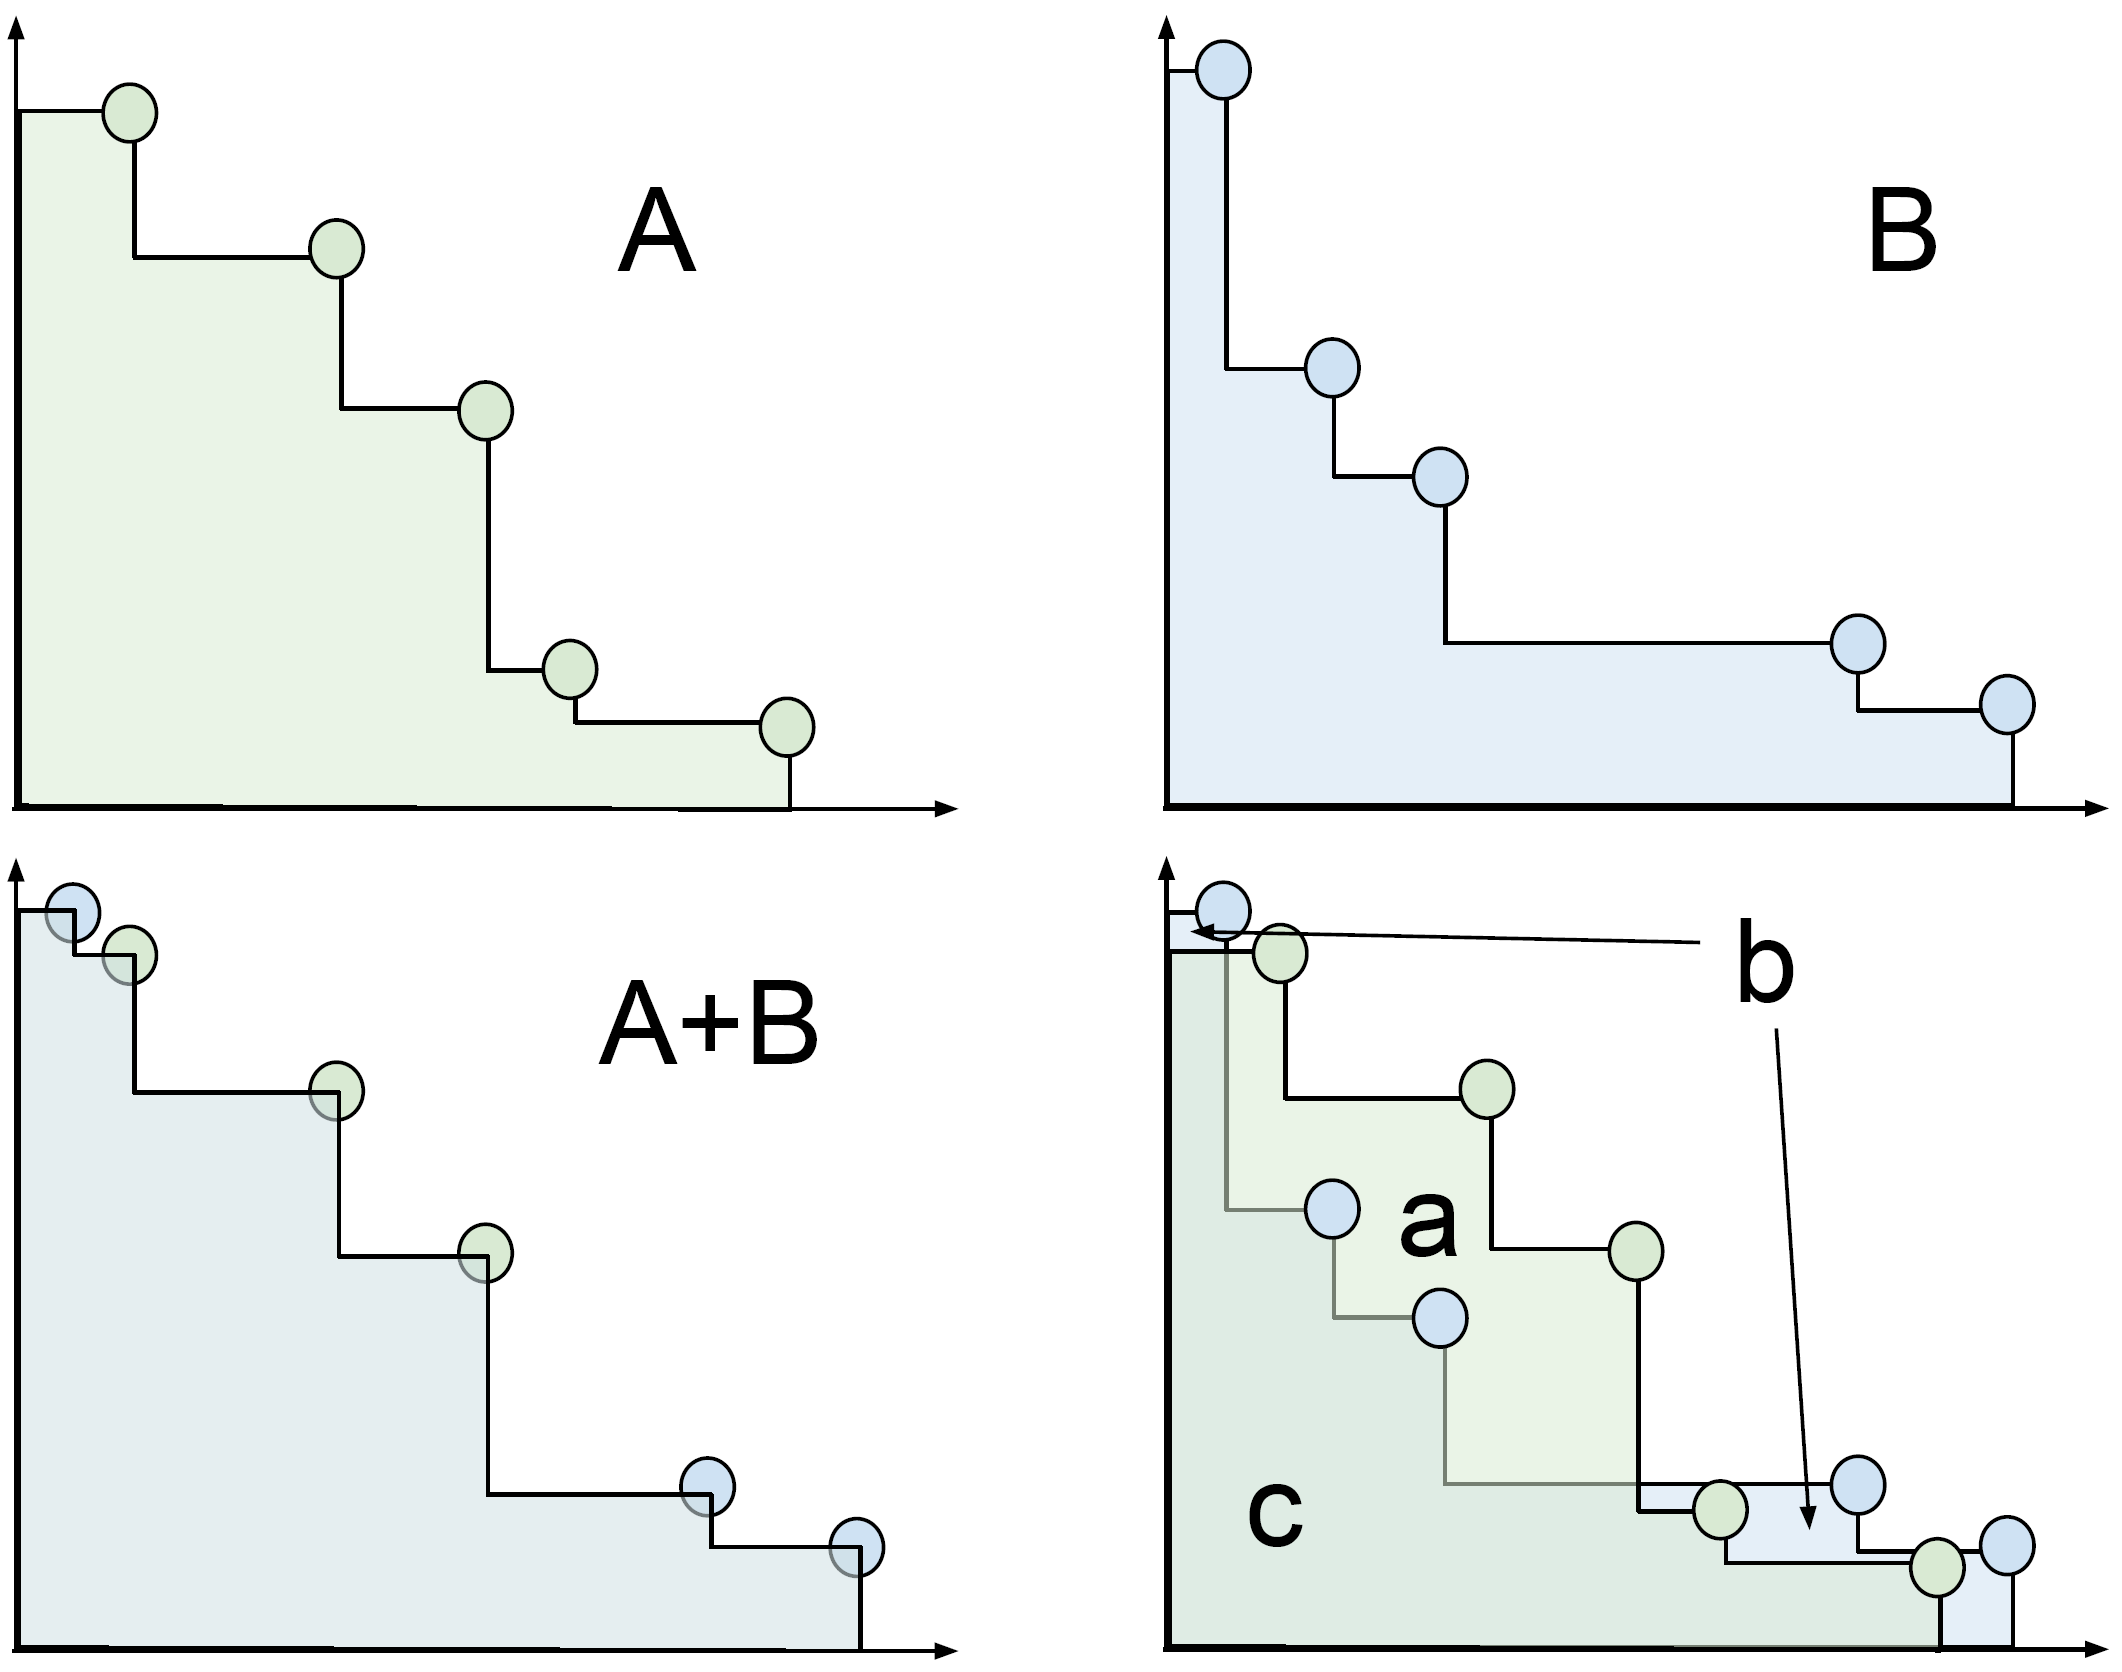
\includegraphics[width=.7\textwidth]{../images/BinaryHypervolume}
\caption[Binary hypervolume indicator]{Depiction of the binary hypervolume indicator. The individual frontiers are shown in the top row: frontier $A$ (left) and frontier $B$ (right). The merged frontier $A+B$ is shown in bottom left - note the absence of points that were dominated when combined. Following the naming of regions as shown in the bottom right figure, the binary hypervolume indicator is equal to
\begin{minipage}{\linewidth}
  \begin{align*}
    I_{H2} (A,B) = \left(\text{area}_a + \text{area}_b + \text{area}_c \right) - \left( \text{area}_b + \text{area}_c \right) = \text{area}_a
  \end{align*}
\end{minipage}%
}
\label{fig:binaryHypervolume}
\end{figure}

I developed a custom algorithm to solve for the hypervolume indicators. The details of the algorithm may be found in \S \ref{chap:appAHypervolumeAlgo}.

\section{Unary distance indicator $I_d$} The unary distance indicator measures the average distance from the frontier to the ideal solution:
\begin{align}
I_d = \frac{1}{|Z|}\sum_{\mathbf{z} \in Z} ||\mathbf{z}^{\text{ideal}} - \mathbf{z} ||
\end{align}
Smaller values of $I_d$ correspond to frontiers that are closer to the ideal solution, which may imply less conflict between objectives. This metric is analogous to the unary distance indicator more commonly used in EMO \cite{czyzzak1998pareto}. Where the metric used here measures the distance to the ideal solution, the traditional metric measures the distance to a reference Pareto frontier.

\section{Unary Spacing Indicator $I_s$} The unary spacing indicator, or Schott's spacing metric \cite{schott1995fault}, computes the standard deviation of the distance between points in the frontier:
\begin{align}
I_s = \sqrt{\frac{1}{|Z|-1} \sum_{\mathbf{z} \in Z} (d_z - \overbar{d})^2}
\end{align}
where
\begin{align}
d_z = \min_{\mathbf{y} \in Z, \mathbf{y} \neq \mathbf{z}} ||\mathbf{z} - \mathbf{y}||
\end{align}
and $\overbar{d}$ is the average over all $d_z$. In EMO, the spacing indicator provides a measure of an algorithm's ability to search the frontier space uniformly. Here, the spacing metric provides a measure of the flexibility afforded to the decision maker, since smaller values of $I_s$ imply less distance between solutions.